\begin{sol}
\begin{enumerate}[label=\textbf{(\alph*)}]
    \item We have three regions to consider: $x<-a$, $-a<x<a$, and $x>a$. For the outer two regions, we have $V=0$, and thus it would be experiencing exponential decay of:
    $$\Psi = \pm e^{-\kappa |x|}$$
    where $\kappa^2 \equiv -\frac{2mE}{\hbar^2}$ and the $\pm$ is dependent on whether the bound state is even or odd. For the middle region, the wavefunction can be either even or odd. If it's even, then it is given by:
    $$\Psi = A_1\cosh(\kappa x)$$
    and if it's odd:
    $$\Psi = A_2\sinh(\kappa x)$$
    Starting with the ground state (even), we can integrate the function from $-a-\epsilon$ to $-a+\epsilon$ with respect to $x$, and taking the limit as $\epsilon\to 0$:
    \begin{align*}
        -\frac{\hbar^2}{2m}\int_{-a-\epsilon}^{-a+\epsilon} \frac{d^2\Psi(x)}{dx^2} \, dx + \int_{-a-\epsilon}^{-a+\epsilon} (-g\delta(x+a))\Psi(x) \, dx &= \int_{-a-\epsilon}^{-a+\epsilon} E\Psi(x) \, dx \\
        -\frac{\hbar^2}{2m}\left(\frac{d\Psi}{dx}\Big|_{-a+\epsilon}-\frac{d\Psi}{dx}\Big|_{-a-\epsilon}\right)-g\delta(-a)&=0 \\
        -\frac{\hbar^2}{2m}\Delta_{-a}\Psi'-g\Psi(-a)&=0 \\ \Delta_{-a}\Psi'&=-\frac{2mg\Psi(-a)}{\hbar^2}
    \end{align*}
We attempt to evaluate the discontinuity function at $x=-a$. Due to symmetry, this will be equal to the discontinuity function at $x=a$. The function however, is continuous at $x=-a$, allowing us to determine $A_1$:
$$\Psi(-a) = A_1\cosh(-\kappa a)=-e^{-\kappa a} \implies A_1 = -\frac{e^{-\kappa a}}{\cosh(-\kappa a)}$$
allowing us to evaluate the discontinuity and solve for $\kappa$
\begin{align*}
    \Delta_{-a}\Psi' &= A\kappa\sinh(-\kappa a)-\left(-\kappa e^{-\kappa a}\right) \\
    -\frac{2mg}{\hbar^2}\left(-e^{-\kappa a}\right)&= \left(-e^{-\kappa a}\right)\kappa \tanh(-\kappa a) - \kappa \left(-e^{-\kappa a}\right) \\
    -\frac{2mg}{\hbar^2} &= \kappa \tanh(-\kappa a) - \kappa \\
    \frac{2mg}{\hbar^2} &= \kappa(1+\tanh(\kappa a) \\
    2\lambda &= a\kappa(1+\tanh(a\kappa))
\end{align*}
We can define $$a\kappa = \sqrt{\frac{2m|E|a^2}{\hbar^2}}=\sqrt{2e}$$
where $e$ is the characteristic energy. This reduces our equation to:
$$2\lambda=\sqrt{2e}(1+\tanh(\sqrt{2e}))$$
Next, we look at our odd states. Everything is the same, except the discontinuity equation is different:
$\kappa$
\begin{align*}
    \Delta_{-a}\Psi' &= A\kappa\cosh(-\kappa a)-\left(-\kappa e^{-\kappa a}\right) \\
    -\frac{2mg}{\hbar^2}\left(-e^{-\kappa x}\right)&= \left(-e^{-\kappa x}\right)\kappa \coth(-\kappa a) - \kappa \left(-e^{-\kappa x}\right) \\
    -\frac{2mg}{\hbar^2} &= \kappa \coth(-\kappa a) - \kappa \\
    \frac{2mg}{\hbar^2} &= \kappa(1+\coth(\kappa a) \\
    2\lambda &= a\kappa(1+\coth(a\kappa))
\end{align*}
And again, our dimensionless equation which we can plot for $e$ is:
$$2\lambda=\sqrt{2e}(1+\coth(\sqrt{2e}))$$
When these two are graphed, we see the energies are both concave up with respect to the dimensionless parameter $\lambda$:
\begin{center}
    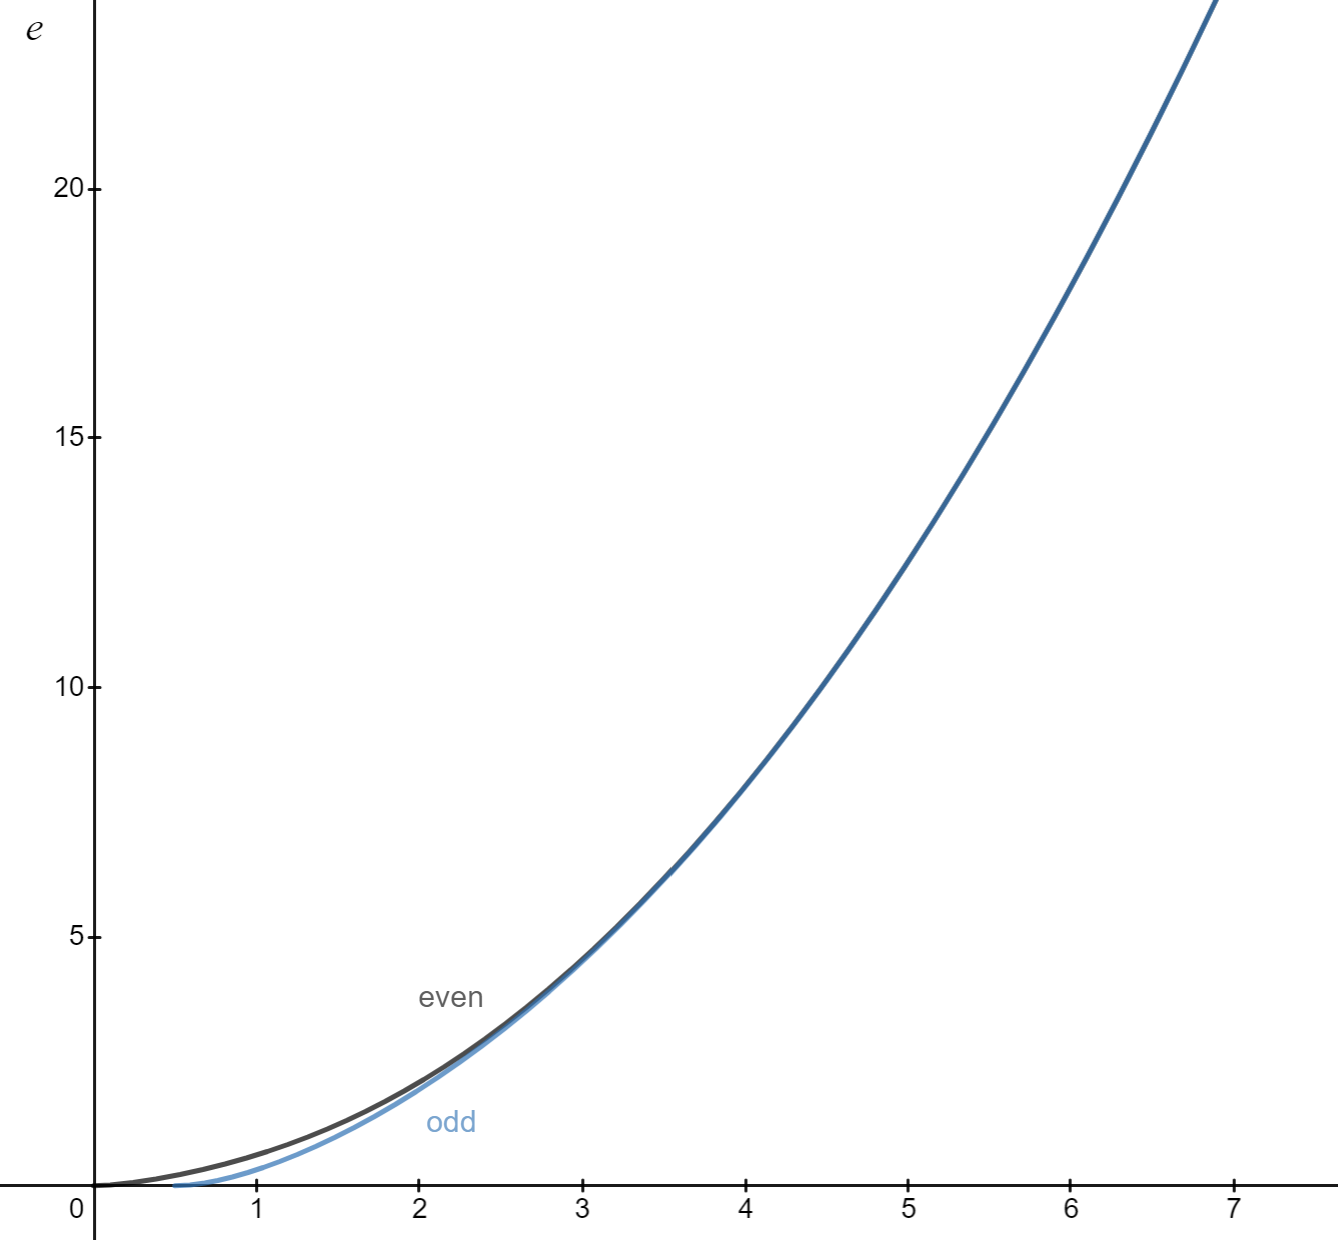
\includegraphics[width=0.6\linewidth]{Images/7-1.png}
\end{center}

% \begin{tikzpicture}
%   \begin{axis}
%     \addplot +[no markers,
%       raw gnuplot,
%       thick,
%       red,
%       empty line = jump % not strictly necessary, as this is the default behaviour in the development version of PGFPlots
%       ] gnuplot {
%       set contour base;
%       set cntrparam levels discrete 0.003;
%       unset surface;
%       set view map;
%       set isosamples 500;
%       splot sqrt(2*y)*(1+tanh(sqrt(2*y)))-2*x;
%     };
%     \addplot +[no markers,
%       raw gnuplot,
%       thick,
%       blue,
%       empty line = jump % not strictly necessary, as this is the default behaviour in the development version of PGFPlots
%       ] gnuplot {
%       set contour base;
%       set cntrparam levels discrete 0.003;
%       unset surface;
%       set view map;
%       set isosamples 500;
%       splot sqrt(2*y)*(3+coth(sqrt(2*y)))-2*x;
%     };
%   \end{axis}
% \end{tikzpicture}

\item As $2a\to \infty$, $a\kappa=\sqrt{2e}$ will approach infinity as well. Since $\tanh(x)$ and $\coth(x)$ have the same asymptotic value, we are left with:
$$\frac{2mga}{\hbar^2}=a\sqrt{\frac{2m|E|}{\hbar^2}} \implies E=-\frac{2mg^2}{\hbar^2}$$
which is the energy of a single delta function potential well. We can intuitively explain this in the framework of locality: The two potential wells are too far away from each other to ``talk'' or communicate with each other so in their own respective surroundings, the wavefunction behaves exactly as if they were the only delta functions.
\vspace{2mm}

However, a more interesting calculation would be the difference in energy as it approaches $2a$ grows large, but not necessarily at infinity. We have:
\begin{align*}
    2\lambda &= \sqrt{2e_1}(1+\tanh(\sqrt{2e_1})) \\
    2\lambda &= \sqrt{2e_2}(1+\coth(\sqrt{2e_2}))
\end{align*}
Subtracting, we can write $e_1=e_2+\Delta e$ where $\Delta e \ll e_1$. Additionally, we can also expand $\tanh(x)\approx 1-e^{-2x}$ and $\coth(x)\approx 1+2e^{-2x}$ for large $x$. This gives:
% \begin{align*}
%     0 &= \sqrt{2(e_2+\Delta e)}(2-e^{-2\sqrt{2(e_2+\Delta e)}}) -\sqrt{2e_2}(2+2e^{-2\sqrt{2e_2}}) \\
%     0 &= \sqrt{2e_2}(2-e^{-\left(\sqrt{2e_2}+\frac{\Delta e}{\sqrt{2e_2}}\right)})+ \frac{\Delta e}{\sqrt{2e_2}}(2-e^{-\left(\sqrt{2e_2}+\frac{\Delta e}{\sqrt{2e_2}}\right)})
%     -\sqrt{2e_2}(2+2e^{-2\sqrt{2e_2}}) \\
%     0 &= 2\sqrt{2e_2}-\sqrt{2e_2}e^{-2\sqrt{2e_2}}-\sqrt{2e_2}e^{-\frac{\Delta e}{\sqrt{2e_2}}} + \frac{2\Delta e}{\sqrt{2 e_2}}-\frac{\Delta e}{\sqrt{2 e_2}}e^{-2\sqrt{2e_2}}-\frac{\Delta e}{\sqrt{2e_2}}e^{-\frac{\Delta e}{\sqrt{2e_2}}}-2\sqrt{2e_2}-2\sqrt{2e_2}e^{-2\sqrt{2e_2}} \\
%     0 &= -3\sqrt{2e_2}e^{-2\sqrt{2e_2}}-\sqrt{2e_2}+\Delta e+\frac{2\Delta e}{\sqrt{2 e_2}}-\frac{\Delta e}{\sqrt{2 e_2}}e^{-2\sqrt{2e_2}}-\frac{\Delta e}{\sqrt{2e_2}}\\
%     0 &= -3\sqrt{2e_2}e^{-2\sqrt{2e_2}}-\sqrt{2e_2}+\Delta e\left(1+\frac{1}{\sqrt{2e_2}}\right)
% \end{align*}
\begin{align*}
    0 &= \sqrt{2(e_2+\Delta e)}(1+\tanh(\sqrt{2e_1}))-\sqrt{2e_2}(1+\coth(\sqrt{2e_1})) \\
    0 &= \sqrt{2e_2}(1+\tanh(\sqrt{2e_1}))+\frac{\Delta e}{\sqrt{2e_2}}(1+\tanh(\sqrt{2e_1}))-\sqrt{2e_2}(1+\coth(\sqrt{2e_1})) \\
    0 &= \sqrt{2e_2}\left(\tanh(\sqrt{2e_1})-\coth(\sqrt{2e_2})\right) + \frac{2\Delta e}{\sqrt{2e_2}} \\
    0 &= -\sqrt{2e_2}\left(e^{-\sqrt{2e_2}}e^{-\frac{\Delta e}{\sqrt{2e_2}}}+2e^{-\sqrt{2e_2}}\right) + \frac{2\Delta e}{\sqrt{2e_2}} \\
    0 &= -3\sqrt{2e_2}e^{-\sqrt{2e_2}} + \frac{2\Delta e}{\sqrt{2e_2}} \\
    \Delta e &= 3e_2e^{-\sqrt{2e_2}}
\end{align*}
We can let $\lambda \approx \sqrt{2e_2}$ to get:
$$\Delta e = \frac{3}{2}\lambda^2e^{-\lambda}$$
We can verify that as $\lambda \to \infty$, we indeed find that $\Delta e \to 0.$
\end{enumerate}
\end{sol}